\chapter{Integral de Riemann}

\section{Introducción}

\begin{quotation}
\marginpar{\adjustimage{max size={0.9\linewidth}{0.9\paperheight}}{imagenes/Riemann.jpeg}\\
Bernhard Riemann 1826-1866. Fue un matemático alemán que realizó contribuciones muy importantes al análisis y la geometría diferencial, algunas de las cuales allanaron el camino para el desarrollo más avanzado de la relatividad general. Su nombre está conectado con la función zeta, la hipótesis de Riemann, la integral de Riemann, el lema de Riemann, las variedades de Riemann, las superficies de Riemann y la geometría de Riemann. 
\flushright{Wikipedia}} 
<< Bernard Riemann recibió su doctorado en 1851, su \emph{Habilitación} en 1854. La habilitación confiere el reconocimiento de la capacidad de crear sustanciales contribuciones en la investigación más allá de la tesis doctoral, y es un prerequisito necesario para ocupar un cargo de profesor en una universidad Alemana. Riemann eligió como tema  de habilitación el problema de las series de Fourier. Su tesis fue titulada \emph{\"Uber die Darstellbarkeit einer Function durch eine trigonometrische Reine} (Sobre la representación de una función por series trigonométricas) y respondía la pregunta:  Cuándo una función definida en el intervalo $(-\pi,\pi)$ puede ser respresentada por la serie trigonométrica $a_0/2+\sum_{n=1}^{\infty}[a_n\cos(nx)+b_n\sen(nx)]$? 
En este trabajo  es donde hallamos   la Integral de Riemann, introducida en una sección corta antes del nucleo principal de la tesis, como parte del trabajo preparatorio que él necesitó desarrollar antes de abordar el problema de representabilidad por series trigonométricas. >> 
\end{quotation}
\begin{flushright}
 David M. Bressoud\\
 A Radical Approach to Lebesgue's Theory of Integration.
\end{flushright}


En este capítulo vamos a desarrollar el concepto de la integral de Riemman. Vamos a exponer la definición de esta integral dada por J. G. Darboux. Discutiremos las propiedades de la intergal, sus alcances y límites. Preparamos así el camino para la introducción de la integral de Lebesgue. 
\marginpar{\adjustimage{max size={0.9\linewidth}{0.9\paperheight}}{imagenes/Darboux.jpg}\\
Jean G. Darboux  1842-1917. Matemático frances. Su trabajo se desarrolló en el análisis (integración, ecuaciones diferenciales parciales) y geometría diferencial (estudio de curvas y superficies).  
\flushright{Wikipedia}} 

Debemos advertir  al alumno que en este curso dejaremos un poco de lado las cuestiones procedimentales de cómo calcular integrales, aspecto que seguramente abordó en cursos anteriores y del cual nos vamos a valer. Tampoco debe esperar que las actividades prácticas se centren en esa dirección. El objetivo del capítulo es recordar y profundizar nuestro conocimiento de la integral de Riemann. No es nuestra intención que el material sea auto contenido. Algunas propiedades sólo las enunciaremos sin demostración pues seguramente estas demostraciones faltantes son parte de curso previos.   Nuestro principal objetivo aquí es discutir la materia conceptual ligada a la integral y cómo es previsible las actividades prácticas estarán orientadas con ese propósito. Por ejemplo, un problema que nos planteamos y que guiará la exposición es el de caracterizar las funciones integrables Riemann. Nos interesa este problema pues  resolverlo entraña el desarrollo de la noción de medida de  Lebesgue, que es el principal concepto abordado en este libro.


La integral encuentra su motivación en diversos problemas. Aparece cuando se busca el centro de masas de un determinado cuerpo, cuando se quieren hallar longitudes de arco, volúmenes, cuando se quiere reconstruir el movimiento de cuerpo conocida su velocidad. En general, cuando se quiere reconstruir determinada propiedad de un conjunto, cuando es conocida esta proiedad sobre regiones infinitesimales.  La integral es utilizada en incontables teorías matemáticas, como ser el mencionado már arriba relativo a las series de Fourier. 

Quizás el 
problema más simple donde aparece la integral es el que utilizaremos como motivación para introducirla y es el concepto de área.  Vamos a tratar de reconstruir este concepto desde su base, esto es analizando la noción de área de figuras tan simples como rectángulos, triángulos, etc. 



\section{Área de figuras elementales planas}\label{sec:area_elem}

  
El cálculo de áreas es necesario en multitud de actividades humanas, por ejemplo con el comercio. La cantidad de muchos productos y servicios se estima en medidas de área, por ejemplo: las telas,  el trabajo de un colocador de pisos,  el precio de la construcción,  el valor de las extensiones de tierra, etc.  
 
 


Por \emph{figuras elementales}\index{figura!elemental} planas nos referimos a rectángulos, triángulos, trapecios, etc. Sin duda el alumno  debe estar  muy familiarizado con las áreas de estas figuras, el área de un rectángulo viene dada por la conocida fórmula $b\times h$, donde $b$ es la base del rectángulo y $h$ su altura.  Ahora bien, ¿Cómo 
se llega a esta fórmula? Porque esta fórmula es apropiada para calcular el precio de un terreno por ejemplo. En esta sección vamos a justificar esta fórmula a partir de algunos hechos elementales.



Vamos a considerar un plano $\mathcal{P}$. En este plano $\mathcal{P}$ supondremos fijada una unidad de longitud.  Pretendemos asignar un área a las figuras, es decir a los subconjuntos, de $\mathcal{P}$. De ahora en más, cómo es usual en esta materia  nos referiremos a \emph{medida}\index{medida} en lugar de área. La medida es un concepto más general  que el concepto de área. No obstante en el contexto en que estamos actualmente son sinónimos.  

Queremos construir pues una función $m$ tal que $m(A)$ represente la medida  de  $A\subset\mathcal{P}$. Ahora bien ¿qué podemos usar de guía con ese objetivo? Si, como dijimos,  desconocemos todas las fórmulas previamente aprendidas, sobre que partimos para construir la medida o área. La respuesta es que tomaremos como principio rector  ciertas propiedades que son deseables  que una medida satisfaga. Ellas son las  siguientes. 




\begin{description}
 \item[Positividad.] debería ser una magnitud no negativa.  
 \item[Invariancia por movimientos rígidos.] Si una región es transformada en otra por medio de un movimiento rígido, ambas regiones deberían tener la misma área. Otra manera de expresar esta propiedad es diciendo que dos figuras \emph{congruentes}\index{congruencia} tienen la misma área. 
 \item[Aditividad.] Si una región $A$ es la unión de cierta cantidad de regiones más chicas mutuamente disjuntas $A_i$, $i=1,\ldots,n$, la medida   de $A$ es la suma de las medidas de los $A_i$.
\end{description}

\begin{figure}[h]
\begin{center}
 
\definecolor{xdxdff}{rgb}{0.49,0.49,1}
\definecolor{zzttqq}{rgb}{0.6,0.2,0}
\definecolor{ududff}{rgb}{0.30,0.30,1}
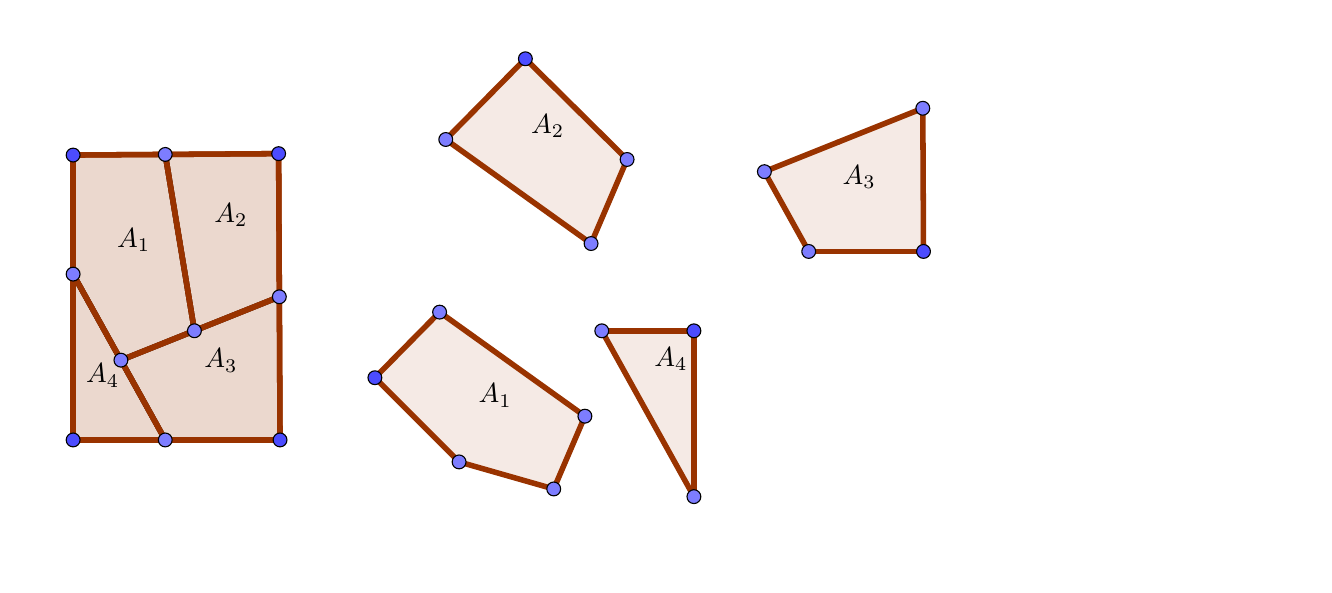
\begin{tikzpicture}[line cap=round,line join=round,x=.9cm,y=.9cm]
\clip(-2.261345665671131,-2.6483801457242535) rectangle (15.749723988011487,4.927708528477943);
\fill[line width=2pt,color=zzttqq,fill=zzttqq,fill opacity=0.10000000149011612] (-1.62,-0.89) -- (-1.62,3.13) -- (1.28,3.15) -- (1.3,-0.89) -- cycle;
\fill[line width=2pt,color=zzttqq,fill=zzttqq,fill opacity=0.10000000149011612] (0.09169246661626662,0.6507662540293884) -- (1.2899992647959808,1.130148511211861) -- (1.28,3.15) -- (-0.3199239037382289,3.1389660420431844) -- cycle;
\fill[line width=2pt,color=zzttqq,fill=zzttqq,fill opacity=0.10000000149011612] (-1.62,1.45) -- (-1.62,3.13) -- (-0.3199239037382289,3.1389660420431844) -- (0.09169246661626662,0.6507662540293884) -- (-0.9454716981132074,0.2358490566037732) -- cycle;
\fill[line width=2pt,color=zzttqq,fill=zzttqq,fill opacity=0.10000000149011612] (-1.62,-0.89) -- (-0.32,-0.89) -- (-1.62,1.45) -- cycle;
\fill[line width=2pt,color=zzttqq,fill=zzttqq,fill opacity=0.10000000149011612] (-0.32,-0.89) -- (-0.9454716981132074,0.2358490566037732) -- (0.09169246661626662,0.6507662540293884) -- (1.2899992647959808,1.130148511211861) -- (1.3,-0.89) -- cycle;
\fill[line width=2pt,color=zzttqq,fill=zzttqq,fill opacity=0.10000000149011612] (8.76,1.77) -- (8.134528301886792,2.8958490566037733) -- (9.171692466616268,3.3107662540293887) -- (10.36999926479598,3.790148511211861) -- (10.38,1.77) -- cycle;
\fill[line width=2pt,color=zzttqq,fill=zzttqq,fill opacity=0.10000000149011612] (3.8264466094067267,-1.199878066911803) -- (2.6385072170133266,-0.011938674518402692) -- (3.551459891609421,0.9136938983359697) -- (5.601939561385962,-0.5546723179904587) -- (5.16194451123264,-1.5814488960049211) -- cycle;
\fill[line width=2pt,color=zzttqq,fill=zzttqq,fill opacity=0.10000000149011612] (5.6888024763961145,1.8814084921516754) -- (6.19715889449669,3.0677137999207305) -- (4.761837661840736,4.4888939366884495) -- (3.638322806619573,3.3497747084781038) -- cycle;
\fill[line width=2pt,color=zzttqq,fill=zzttqq,fill opacity=0.10000000149011612] (7.14,0.65) -- (5.84,0.65) -- (7.14,-1.69) -- cycle;
\draw [line width=2pt,color=zzttqq] (-1.62,-0.89)-- (-1.62,3.13);
\draw [line width=2pt,color=zzttqq] (-1.62,3.13)-- (1.28,3.15);
\draw [line width=2pt,color=zzttqq] (1.28,3.15)-- (1.3,-0.89);
\draw [line width=2pt,color=zzttqq] (1.3,-0.89)-- (-1.62,-0.89);
\draw [line width=2pt] (-1.62,1.45)-- (-0.32,-0.89);
\draw [line width=2pt] (-0.9454716981132074,0.2358490566037732)-- (1.2899992647959808,1.130148511211861);
\draw [line width=2pt] (-0.3199239037382289,3.1389660420431844)-- (0.09169246661626662,0.6507662540293884);
\draw [line width=2pt,color=zzttqq] (0.09169246661626662,0.6507662540293884)-- (1.2899992647959808,1.130148511211861);
\draw [line width=2pt,color=zzttqq] (1.2899992647959808,1.130148511211861)-- (1.28,3.15);
\draw [line width=2pt,color=zzttqq] (1.28,3.15)-- (-0.3199239037382289,3.1389660420431844);
\draw [line width=2pt,color=zzttqq] (-0.3199239037382289,3.1389660420431844)-- (0.09169246661626662,0.6507662540293884);
\draw [line width=2pt,color=zzttqq] (-1.62,1.45)-- (-1.62,3.13);
\draw [line width=2pt,color=zzttqq] (-1.62,3.13)-- (-0.3199239037382289,3.1389660420431844);
\draw [line width=2pt,color=zzttqq] (-0.3199239037382289,3.1389660420431844)-- (0.09169246661626662,0.6507662540293884);
\draw [line width=2pt,color=zzttqq] (0.09169246661626662,0.6507662540293884)-- (-0.9454716981132074,0.2358490566037732);
\draw [line width=2pt,color=zzttqq] (-0.9454716981132074,0.2358490566037732)-- (-1.62,1.45);
\draw [line width=2pt,color=zzttqq] (-1.62,-0.89)-- (-0.32,-0.89);
\draw [line width=2pt,color=zzttqq] (-0.32,-0.89)-- (-1.62,1.45);
\draw [line width=2pt,color=zzttqq] (-1.62,1.45)-- (-1.62,-0.89);
\draw [line width=2pt,color=zzttqq] (-0.32,-0.89)-- (-0.9454716981132074,0.2358490566037732);
\draw [line width=2pt,color=zzttqq] (-0.9454716981132074,0.2358490566037732)-- (0.09169246661626662,0.6507662540293884);
\draw [line width=2pt,color=zzttqq] (0.09169246661626662,0.6507662540293884)-- (1.2899992647959808,1.130148511211861);
\draw [line width=2pt,color=zzttqq] (1.2899992647959808,1.130148511211861)-- (1.3,-0.89);
\draw [line width=2pt,color=zzttqq] (1.3,-0.89)-- (-0.32,-0.89);
\draw [line width=2pt,color=zzttqq] (8.76,1.77)-- (8.134528301886792,2.8958490566037733);
\draw [line width=2pt,color=zzttqq] (8.134528301886792,2.8958490566037733)-- (9.171692466616268,3.3107662540293887);
\draw [line width=2pt,color=zzttqq] (9.171692466616268,3.3107662540293887)-- (10.36999926479598,3.790148511211861);
\draw [line width=2pt,color=zzttqq] (10.36999926479598,3.790148511211861)-- (10.38,1.77);
\draw [line width=2pt,color=zzttqq] (10.38,1.77)-- (8.76,1.77);
\draw [line width=2pt,color=zzttqq] (3.8264466094067267,-1.199878066911803)-- (2.6385072170133266,-0.011938674518402692);
\draw [line width=2pt,color=zzttqq] (2.6385072170133266,-0.011938674518402692)-- (3.551459891609421,0.9136938983359697);
\draw [line width=2pt,color=zzttqq] (3.551459891609421,0.9136938983359697)-- (5.601939561385962,-0.5546723179904587);
\draw [line width=2pt,color=zzttqq] (5.601939561385962,-0.5546723179904587)-- (5.16194451123264,-1.5814488960049211);
\draw [line width=2pt,color=zzttqq] (5.16194451123264,-1.5814488960049211)-- (3.8264466094067267,-1.199878066911803);
\draw [line width=2pt,color=zzttqq] (5.6888024763961145,1.8814084921516754)-- (6.19715889449669,3.0677137999207305);
\draw [line width=2pt,color=zzttqq] (6.19715889449669,3.0677137999207305)-- (4.761837661840736,4.4888939366884495);
\draw [line width=2pt,color=zzttqq] (4.761837661840736,4.4888939366884495)-- (3.638322806619573,3.3497747084781038);
\draw [line width=2pt,color=zzttqq] (3.638322806619573,3.3497747084781038)-- (5.6888024763961145,1.8814084921516754);
\draw [line width=2pt,color=zzttqq] (7.14,0.65)-- (5.84,0.65);
\draw [line width=2pt,color=zzttqq] (5.84,0.65)-- (7.14,-1.69);
\draw [line width=2pt,color=zzttqq] (7.14,-1.69)-- (7.14,0.65);
\draw (-1.1356538123159674,2.2366014415507594) node[anchor=north west] {$A_1$};
\draw (3.9651373981996176,0.03798454046645946) node[anchor=north west] {$A_1$};
\draw (0.23628313396063827,2.5883801457242477) node[anchor=north west] {$A_2$};
\draw (4.703872676963944,3.83719454554013) node[anchor=north west] {$A_2$};
\draw (0.09557165229124281,0.5304747263093427) node[anchor=north west] {$A_3$};
\draw (9.101106479132552,3.1160482019844795) node[anchor=north west] {$A_3$};
\draw (-1.5753771925328282,0.31940750380524985) node[anchor=north west] {$A_4$};
\draw (6.445177262622713,0.5480636615180171) node[anchor=north west] {$A_4$};
\begin{scriptsize}
\draw [fill=ududff] (-1.62,-0.89) circle (2.5pt);
\draw [fill=ududff] (-1.62,3.13) circle (2.5pt);
\draw [fill=ududff] (1.28,3.15) circle (2.5pt);
\draw [fill=ududff] (1.3,-0.89) circle (2.5pt);
\draw [fill=xdxdff] (-1.62,1.45) circle (2.5pt);
\draw [fill=xdxdff] (-0.32,-0.89) circle (2.5pt);
\draw [fill=xdxdff] (-0.9454716981132074,0.2358490566037732) circle (2.5pt);
\draw [fill=xdxdff] (1.2899992647959808,1.130148511211861) circle (2.5pt);
\draw [fill=xdxdff] (-0.3199239037382289,3.1389660420431844) circle (2.5pt);
\draw [fill=xdxdff] (0.09169246661626662,0.6507662540293884) circle (2.5pt);
\draw [fill=xdxdff] (8.76,1.77) circle (2.5pt);
\draw [fill=xdxdff] (8.134528301886792,2.8958490566037733) circle (2.5pt);
\draw [fill=xdxdff] (10.36999926479598,3.790148511211861) circle (2.5pt);
\draw [fill=ududff] (10.38,1.77) circle (2.5pt);
\draw [fill=xdxdff] (3.8264466094067267,-1.199878066911803) circle (2.5pt);
\draw [fill=ududff] (2.6385072170133266,-0.011938674518402692) circle (2.5pt);
\draw [fill=xdxdff] (3.551459891609421,0.9136938983359697) circle (2.5pt);
\draw [fill=xdxdff] (5.601939561385962,-0.5546723179904587) circle (2.5pt);
\draw [fill=xdxdff] (5.16194451123264,-1.5814488960049211) circle (2.5pt);
\draw [fill=xdxdff] (5.6888024763961145,1.8814084921516754) circle (2.5pt);
\draw [fill=xdxdff] (6.19715889449669,3.0677137999207305) circle (2.5pt);
\draw [fill=ududff] (4.761837661840736,4.4888939366884495) circle (2.5pt);
\draw [fill=xdxdff] (3.638322806619573,3.3497747084781038) circle (2.5pt);
\draw [fill=ududff] (7.14,0.65) circle (2.5pt);
\draw [fill=xdxdff] (5.84,0.65) circle (2.5pt);
\draw [fill=xdxdff] (7.14,-1.69) circle (2.5pt);
\end{scriptsize}
\end{tikzpicture}


 \caption{El área del rectángulo es la suma de sus partes}\label{fig:rect_descop} 
\end{center}
\end{figure}

Utilizando la segunda y tercer propiedad se pueden relacionar el área del rectángulo de la figura \ref{fig:rect_descop} con las cuatro regiones en la que es dividido.

Como veremos a lo largo de la materia la propiedad de aditividad debe ser estudiada con cuidado, esto ocurre por las intrincadas maneras en que una región puede ser unión de otras regiones. A lo largo de esta materia elaboraremos una  teoría que nos dará una descripción  precisa de a que conjuntos podemos asignarle una medida de modo que las propiedades previas sean consistentes. 

Por el momento veamos como las propiedades anteriores determinan practicamente de manera unívoca la medida de regiones elementales planas.  


Hablando de propiedades de la medida, supongamos que $A$ y $B$ son dos regiones con $A\subset B$. Entonces como $B=A\cup (B-A)$ y por la propiedad de aditividad y positividad

\[
 m(B)=m(A)+m(B-A)\geq m(A).
\]

Descubrimos así que nuestra medida deberá tener adicionalmente la siguiente propiedad:
\begin{description}
 \item[Monotonía.] Si $A\subset B$ entonces $m(A)\leq m(B)$. 
\end{description}
\marginpar{ Podríamos por ejemplo elegir el círculo de radio uno como unidad de área. Así ya no tendríamos el problema de ese número raro $\pi$ que aparece en la fórmula del área del círculo. ¡El área de cualquier círculo sería igual a su radio al cuadrado! Claro que aparecería $\pi$  en la fórmula del área del cuadrado de lado 1. Nos tapamos los pies y se destapa el cuerpo.}
Es claro que si logramos construir una medida que satisfaga las propiedades anteriores cualquier multiplo por un número real positivo  de ella seguirá cumpliendo las propiedades. Esto es una manera de expresar el hecho que podemos usar diferentes unidades de medición. Esta cuestión se sortea proponiendo la unidad de medida. Esta unidad es completamente arbitraria, ud. podría elegir su figura plana preferida como unidad de área.   Cómo es habitual, elijamos el cuadrado cuyos lados miden la unidad de longitud supuesto que esta unidad fue previamente establecida. 


Supongamos ahora que tenemos un rectángulo $R$ de un lado igual a la unidad y el otro de longitud racional $n/m$, $n,m\in\mathbb{N}$. Veamos que las propiedades de las medidas determinan el área de este rectángulo. Sea $Q$ un cuadrado de lados iguales a 1. Luego $m(Q)=1$, por suposición.  Primero observar que si dividimos un lado de $Q$ en $m$ segmentos iguales de longitud $1/m$, queda dividido el cuadrado en $m$ rectángulos $R_1,\ldots,R_m$ (ver figura en el margen), todos ellos  congruentes entre si, de modo que todos tienen la misma medida, digamos $m(R_1)$.  De modo que por la aditividad debe ocurrir que $m(R_1)=\cdots =m(R_m))=1/m$. Recordemos nuestra pretención de inferir la medida de un rectángulo $R$ de lado 1 y otro $n/m$. Este rectángulo esta compuesto de $n$ rectángulos congruentes a los $R_i$, $i=1,\ldots,m$, nuevamente por la aditividad inferimos que $m(R)=n/m$. Notar que $n/m$ es la base por la altura de $R$.

Sea ahora una rectángulo $R$ con un lado unidad y el otro un real cualquiera $l>0$. Existen sendas sucesiones $0<q_k,p_k\in\mathbb{Q}$, $k\in\mathbb{N}$, tales que $q_1\leq q_2\leq\cdots \leq l \leq \cdots\leq p_2\leq p_1$ y $\lim_{k\to\infty}q_k =\lim_{k\to\infty} p_k=l$. Consideremos una dos sucesiones de rectángulos $R_k$ y $S_k$ que comparten el lado de $R$ igual a la unidad, mientras que los otros lados de $R_k$ y $S_k$ son iguales a $q_k$ y $p_k$ respectivamente. Luego por la monotonía
\[
 q_k=m(R_k)\leq m(R) \leq m(S_k)\leq p_k.
\]
Tomando límite cuando $k\to\infty$ inferimos que $m(R)=l$. 




\marginpar{
 
\definecolor{xdxdff}{rgb}{0.49,0.49,1}
\definecolor{zzttqq}{rgb}{0.6,0.2,0}
\definecolor{ududff}{rgb}{0.30,0.30,1}
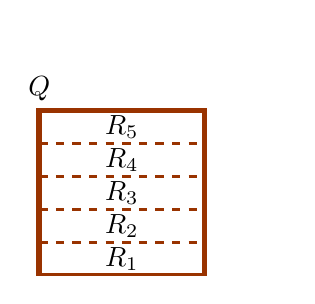
\begin{tikzpicture}[x=2.1cm,y=2.1cm]
\clip(-0.07,0) rectangle (1.5,1.5);
\draw [line width=2pt,color=zzttqq] (0,0) -- (1,0) -- (1,1) -- (0,1) -- cycle;
\draw [line width=1pt,color=zzttqq, dashed] (0,.2)--(1,.2);
\draw [line width=1pt,color=zzttqq, dashed] (0,.4)--(1,.4);
\draw [line width=1pt,color=zzttqq, dashed] (0,.6)--(1,.6);
\draw [line width=1pt,color=zzttqq, dashed] (0,.8)--(1,.8);
\draw (0,1) node[anchor=south] {$Q$};
\draw (0.5,.1) node[anchor=center] {$R_1$};
\draw (0.5,.3) node[anchor=center] {$R_2$};
\draw (0.5,.5) node[anchor=center] {$R_3$};
\draw (0.5,.7) node[anchor=center] {$R_4$};
\draw (0.5,.9) node[anchor=center] {$R_5$};



\end{tikzpicture}
\\
 Descomposición del cuadrado $Q$
 } 
A partir de las propiedades fundamentales que postulamos para la medida o área inferimos la famosa fórmula del área de un rectángulo en el caso que uno de los lados sea igual a la unidad. Si ahora tenemos un rectángulo arbitrario, hay que fijar un lado y repetir el análisis previo con el segundo lado. Se llega de este modo a justificar la fórmula del área para un  rectángulo arbitrario. 


\begin{figure}[h]
 \begin{center}
 

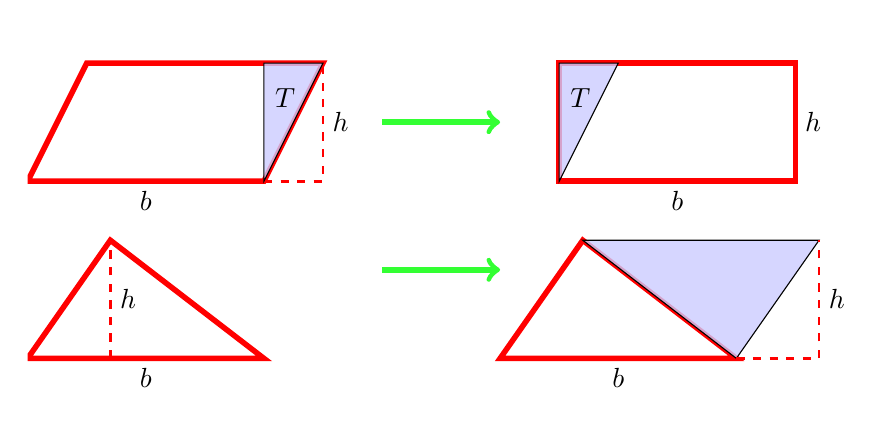
\begin{tikzpicture}[x=1.5cm,y=1.5cm]
\clip(0,-2) rectangle (7,1.3);
\tikzstyle{ColorRell1} = [fill=blue!20,fill opacity=0.8]
\tikzstyle{ColorLine1} = [color=red]
\tikzstyle{ColorLine2} = [color=green!80]


\draw [line width=2pt,ColorLine1] (0,0) -- (2,0) -- (2.5,1) -- (0.5,1) -- cycle;
\draw [line width=1pt,ColorLine1, dashed] (2,0)--(2.5,0)--(2.5,1);

\draw (2.5,0.5) node[anchor=west] {$h$};
\draw (1,0) node[anchor=north] {$b$};
\draw[arrows=->,line width=2pt, ColorLine2](3,0.5)--(4,0.5);

\filldraw[ColorRell1](2,0)--(2,1)--(2.5,1)--cycle;

\draw (2.18,.7) node[anchor=center] {$T$};



\draw [line width=2pt,ColorLine1] (4.5,0) -- (6.5,0) -- (6.5,1) -- (4.5,1) -- cycle;


\draw (6.5,0.5) node[anchor=west] {$h$};
\draw (5.5,0) node[anchor=north] {$b$};

\filldraw[ColorRell1](4.5,0)--(5,1)--(4.5,1)--cycle;

\draw (4.68,.7) node[anchor=center] {$T$};

\draw [line width=2pt,ColorLine1] (0,-1.5) -- (2,-1.5) -- (.7,-0.5) -- cycle;
\draw[arrows=->,line width=2pt, ColorLine2](3,-0.75)--(4,-0.75);
\draw [line width=1pt,ColorLine1, dashed] (.7,-1.5)--(0.7,-0.5);
\draw (0.7,-1) node[anchor=west] {$h$};

\draw (1,-1.5) node[anchor=north] {$b$};


\draw [line width=2pt,ColorLine1,shift={(4,0)}] (0,-1.5) -- (2,-1.5) -- (.7,-0.5) -- cycle;
\filldraw[ColorRell1,shift={(4,0)}](2,-1.5)--(.7,-0.5)--(2.7,-0.5)--cycle;
\draw [line width=1pt,ColorLine1,shift={(4,0)}, dashed] (2,-1.5)--(2.7,-1.5)--(2.7,-.5);
\draw (6.7,-1) node[anchor=west] {$h$};

\draw (5,-1.5) node[anchor=north] {$b$};














\end{tikzpicture} 
 \end{center}
 \caption{Áreas de otras figuras elementales.}\label{fig:paral-trig}
\end{figure}

En la figura \ref{fig:paral-trig} se muestra como relacionar el área de un paralelepípedo con la de un rectángulo y la de un triángulo con la de un paralelepípedo para inferir las conocidas fórmulas para estas figuras.



\section{Integral de Riemann}

En esta sección abordaremos el problema del área de regiones planas. Vamos a contextualizarnos dentro del marco conceptual que nos brinda la geometría analítica. Mediante coordenadas cartesianas ortogonales los puntos del plano se identifican con pares ordenados $(x,y)\in\mathbb{R}^2$ y el plano con el conjunto $\rr^2$.  Nuestro propósito es entonces definir la medida de subconjuntos de $\mathbb{R}^2$. La geometría analítica abre así nuevas posibilidades para abordar el problema del área. 

Nuestra primera aproximación será la que propuso Bernhard Riemann en 1854, pero seguiremos  el enfoque de Jean Darboux. En esta parte de nuestra exposición consideraremos subconjuntos de $\mathbb{R}^2$ de un tipo especial, concretamente a conjuntos que quedan encerrados entre la gráfica de una función y del eje coordenadas $x$. Esto nos lleva alconcepto de integral. 


\begin{definicion}[Partición]{} Sea $[a,b]$ un intervalo. Una {\em partición}\index{Partición} $P$ es un conjunto ordenado y finito de puntos, donde el primer elemento es $a$ y el último $b$. Es decir $P=\{x_0,x_1,\ldots,x_n\}$, donde $a=x_0<x_1<\cdots<x_n=b$. 
 
\end{definicion}




\begin{definicion}[Sumas de Darboux]{} Sea $f:[a,b]\to\mathbb{R}$ una función acotada y $P=\{x_0,x_1,\ldots,x_n\}$ una partición de $[a,b]$. Consideremos las siguientes magnitudes
\begin{equation}\label{eq:Mi-mi}
 \begin{split}
    m_i&:=\inf\{f(x)| x\in [x_{i-1},x_i]\}\\
    M_i&:=\sup\{f(x)| x\in [x_{i-1},x_i]\}\\
 \end{split}
\end{equation}

Definimos la \emph{Suma superior de Darboux}\index{Suma superior} como
\[
 \overline{S}(P,f)=\sum_{i=1}^nM_i(x_i-x_{i-1}),
\]
y la \emph{Suma inferior de Darboux}\index{Suma inferiorr} como
\[
 \underline{S}(P,f)=\sum_{i=1}^nm_i(x_i-x_{i-1}),
\] 
\end{definicion}
\marginpar{
  \begin{center}
    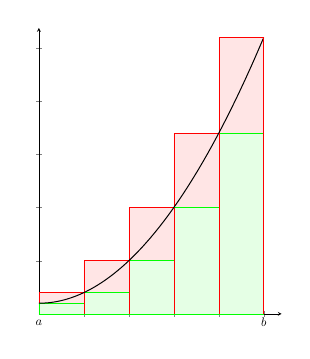
\begin{tikzpicture}[scale=0.45]
\begin{axis}[
    xtick={0,...,5},ytick={5,10,15,20,25},
    y=0.3cm, xmax=5.4,ymax=26.9,ymin=0,xmin=0,
    enlargelimits=true,
    axis lines=middle,
    clip=false,yticklabels=\empty,xticklabels=\empty,
    ]
\addplot+[color=red,fill=red!10!white,const plot, mark=none]
    coordinates {(0,2) (1,5) (2,10) (3,17) (4,26) (5,26)}\closedcycle;
\addplot+[color=green,fill=green!10!white,const plot, mark=none]
    coordinates {(0,1) (1,2) (2,5) (3,10) (4.0,17) (5,17)}\closedcycle;
\addplot[smooth, thick,domain=0:5]{1+x^2};
\addplot[const plot,domain=0:5,color=red] coordinates {(1,0) (1,2)};
\addplot[const plot,domain=0:5,color=red] coordinates {(2,0) (2,5)};
\addplot[const plot,domain=0:5,color=red] coordinates {(3,0) (3,10)};
\addplot[const plot,domain=0:5,color=red] coordinates {(4,0) (4,17)};
\addplot[const plot,domain=0:5,color=red] coordinates {(5,0) (5,26)};
\addplot[color=black] coordinates {(0,-0.8)} node {$a$};
\addplot[color=black] coordinates {(5,-0.8)} node {$b$};

\end{axis}
\end{tikzpicture}
    Sumas de Darboux. 
  \end{center}
}

\begin{lema}[Monotonía sumas de Darboux]{}  Sea $f:[a,b]\to\mathbb{R}$ una función acotada y $P=\{x_0,x_1,\ldots,x_n\}$ una partición de $[a,b]$. Supongamos que $P'$ es otra partición que tiene un punto más que $P$. Entoces
 \[
  \underline{S}(P',f)\geq \underline{S}(P,f)\quad\text{y}\quad \overline{S}(P',f)\leq \overline{S}(P,f)
 \]
\end{lema}

\begin{proof} Supongamos que 
\[P=\{x_0,x_1,\ldots,x_n\},\]
\[P'=\{x_0,x_1,\ldots,x_{i-1},x^*,x_{i},x_n\}.\]
Sean $m_i,M_i$ como en \eqref{eq:Mi-mi} 
y es escribamos 
\[
 \begin{split}
    m'_i&:=\inf\{f(x)| x\in [x_{i-1},x^*]\}\\
    M'_i&:=\sup\{f(x)| x\in [x_{i-1},x^*]\}\\
    m''_i&:=\inf\{f(x)| x\in [x^*,x_i]\}\\
    M''_i&:=\sup\{f(x)| x\in [x^*,x_i]\}\\
 \end{split}
\]
 Valen las relaciones $m_i\leq m'_i$, $m_i\leq m''_i$, $M_i'\leq M_i$ y $M''_i\leq M_i$. Entonces
 \begin{multline*}
 \underline{S}(P,f)=\sum_{i=1}^nm_i(x_i-x_{i-1})\\=
 m_1(x_1-x_0)+\cdots+m_i(x^*-x_{i-1})+m_i(x_i-x^*)+\cdots++m_n(x_n-x_{n-1})\\
 \leq m_1(x_1-x_0)+\cdots+m'_i(x^*-x_{i-1})+m''_i(x_i-x^*)+\cdots++m_n(x_n-x_{n-1})\\
 \leq \underline{S}(P',f).
\end{multline*}
 Obviamente la demostración para las sumas superiores es completamente análoga.  
\end{proof}

Usando inducción podemos generalizar el resultado anterior como muestra el siguiente ejercicio.

\begin{ejercicio}{ej:sumas-darboux-mon} Sea $f:[a,b]\to\mathbb{R}$ una función acotada y $P,P'$ particiones de $[a,b]$ con $P\subset P'$. Demostrar que 
  \[
  \underline{S}(P,f)\leq \underline{S}(P',f)\quad\text{y}\quad \overline{S}(P',f)\leq \overline{S}(P,f).
 \]
 Inferir que para cualesquiera $P,P'$ (sin importar que una este o no contenida dentro de la otra)
   \[
\underline{S}(P,f)\leq \overline{S}(P,f).
 \]
 
\end{ejercicio}

\begin{definicion}[Funciones integrables]{def:int_riemann} Sea $f:[a,b]\to\mathbb{R}$ una función acotada. Diremos que $f$ es {\em integrable Riemann} \index{Integrable!Riemann} si 
\begin{equation}\label{eq:integrable}
 \sup\left\{\underline{S}(P,f)| P \text{ partición de }[a,b]\right\}=\inf\left\{\overline{S}(P,f)| P \text{ partición de }[a,b]\right\}
\end{equation}
En caso que $f$ sea integrable Riemann llamamos {\em integral de Riemann} \index{integral!Riemann} entre $a$ y $b$ de $f$ al valor de los dos miembros de \eqref{eq:integrable} y este número se denota
\[
(\mathop{R})\int_a^bf(x)dx. 
\]
Cuando no haya lugar a confusión, por ejemplo a lo largo de este capítulo, omitiremos el símbolo $(\mathop{R})$ en la integral.
\end{definicion}



\begin{teorema}[Propiedades elementales de la integral]{teo:prop_elem} Sean $f,g:[a,b]\to\mathbb{R}$ integrables, $\alpha,\beta\in\mathbb{R}$ y $c\in (a,b)$. Entonces
\begin{description}
 \item[Linealidad] $\alpha f+\beta g$ es integrable y 
 \[
  \int_a^b\alpha f(x)+\beta g(x)dx=\alpha \int_a^bf(x)dx+\beta\int_a^b g(x)dx.
 \]
 \item[Monotonía] Si $f(x)\leq g(x)$  para $x\in [a,b]$ entonces 
 \[
  \int_a^b f(x)dx\leq \int_a^b g(x)dx.
 \]
 \item[Aditividad del Intervalo]  \[
  \int_a^b  f(x)dx= \int_a^cf(x)dx+\int_c^b f(x)dx.
 \]
\end{description}


\end{teorema}

\begin{proof} Fue dada en cursos previos y la omitiremos aquí. 
\end{proof}


\begin{observa} Las propiedadades anteriores son compatibles con las propiedades que habíamos propuesto para el concepto de área en la sección  \ref{sec:area_elem}.
\end{observa}



Es útil tener un símbolo que nos represente el supremo y el ínfimo en la Definición \ref{def:int_riemann}.

\begin{definicion}[Integrables de Darboux]{def:int_dar}
 Sea $f:[a,b]\to\mathbb{R}$ una función acotada. Definimos la integral \emph{superior e inferior de Darboux} \index{integral!Darboux} como
\begin{equation}\label{eq:darboux_sup}
 (\mathop{D})\overline{\int_a^b}f(x)dx=\inf\left\{\overline{S}(P,f)| P \text{ partición de }[a,b]\right\}.
 \end{equation}
y
\begin{equation}\label{eq:darboux_inf}
 (\mathop{D})\underline{\int_a^b}f(x)dx=\sup\left\{\underline{S}(P,f)| P \text{ partición de }[a,b]\right\}.
 \end{equation}
\end{definicion}

Apelando a estos conceptos se tiene que $f$ es integrable Riemann si y sólo si 
\begin{equation}\label{eq:darboux_riemann}
 (\mathop{D})\overline{\int_a^b}f(x)dx= (\mathop{D})\underline{\int_a^b}f(x)dx .
 \end{equation}

 
\begin{teorema}[Primer criterio de integrabilidad]{}  Sea $f:[a,b]\to\mathbb{R}$ una función acotada. Entonces  $f$ es integrable si y solo si para todo $\epsilon>0$ existe una partición $P$ tal que 
\begin{equation}\label{eq:Crit1Int}
 \overline{S}(P;f)-\underline{S}(P;f)<\epsilon.
\end{equation}
 
\end{teorema}

\begin{demo} Veamos la parte ``solo si''. Si $f$ es integrable satisface \eqref{eq:integrable}. Si $\varepsilon>0$, usando la caracterización \eqref{lem:sup-inf-carac} (\textcolor{red}{debería haber una intro con estas propiedades}) tenemos que existen particiones $P'$ y $P''$ tales que:


\begin{eqnarray*}
 \int_a^bf(x)dx&\leq \overline{S}(P';f)&<\int_a^bf(x)dx+\frac{\varepsilon}{2},\\
 \int_a^bf(x)dx-\frac{\varepsilon}{2}&<\underline{S}(P'';f)&\leq\int_a^bf(x)dx.
\end{eqnarray*}

Sea ahora la partición $P=P'\cup P''$. Por el ejercicio \eqref{ej:sumas-darboux-mon} tenemos que:
\begin{multline*}
 \overline{S}(P;f)-\frac{\varepsilon}{2}\leq \overline{S}(P';f)-\frac{\varepsilon}{2}<\int_a^bf(x)dx<\underline{S}(P'';f)+\frac{\varepsilon}{2}
 \leq \underline{S}(P;f)+\frac{\varepsilon}{2}
\end{multline*}
Así tenemos \eqref{eq:Crit1Int}. 

Asumamos ahora que se satisface \eqref{eq:Crit1Int}. Entonces 

 \[
   (\mathop{D})\overline{\int_a^b}f(x)dx\leq \overline{S}(P;f)<
   \underline{S}(P;f)+\varepsilon<(\mathop{D})\underline{\int_a^b}f(x)dx +\varepsilon.
 \]
\end{demo}


\begin{ejemplo}{ejemplo:integral-de-x} Sea $0\leq a<b$ veamos que 
\[
 \int_a^b x dx=\frac{b^2}{2}-\frac{a^2}{2}.
\]
\begin{demo}
Sea $n \in \nn$.
Consideramos particiones uniformes $P_n=\{x_0,x_1,\ldots,x_n\}$ tales que
\[x_k=a+\frac{k}{n}(b-a),\;\;  k=0,1,\ldots,n.\]
Definimos
\[\begin{split}
m_i&=\inf\limits_{[x_{i-1},x_i]}f(x)=x_{i-1}=a+\frac{i-1}{n}(b-a),
\\
M_i&=\sup\limits_{[x_{i-1},x_i]}f(x)=x_{i}=a+\frac{i}{n}(b-a).
\end{split}\]
Luego
\[
\overline{S}(f,P_n)-\underline{S}(f,P_n)=
\sum\limits_{i=0}^{n-1} (M_i-m_i)(x_i-x_{i-1})=
\sum\limits_{i=0}^{n-1}  
\frac{b-a}{n}\frac{b-a}{n}=\frac{(b-a)^2}{n}
\]
y tomando $n$ suficientemente grande vemos que $\overline{S}(f,P_n)-\underline{S}(f,P_n)$ es menor que $\epsilon$.

Hasta aqu\'i, por aplicaci\'on del Primer Criterio de Integrabilidad,  hemos probado que $f(x)=x$ es integrable. 

Para justificar el valor de la integral operamos del siguiente modo
\[
\begin{split}
\overline{S}(f,P_n)=&
\sum\limits_{i=0}^{n-1} M_i(x_i-x_{i-1})
\\
=&\sum\limits_{i=0}^{n-1} x_i(x_i-x_{i-1})=\sum\limits_{i=0}^{n-1}
\left(a+\frac{i}{n}(b-a) \right)\frac{b-a}{n}
\\
=&a(b-a)+\left(\frac{b-a}{n} \right)^2\sum\limits_{i=0}^{n-1} i
\\
=& a(b-a)+\left(\frac{b-a}{n} \right)^2 \frac{n(n+1)}{2}
\\
=&(b-a)\left(a+\frac{n+1}{2n} (b-a)\right).
\end{split}
\]
Ahora observamos que 
$\lim\limits_{n \to \infty} \overline{S}(f,P_n)=\frac{b^2-a^2}{2}$
Se llega a la misma conclusi\'on con $\underline{S}(f,P_n)$.

Luego, como 
\[
\underline{S}(f,P_n)\leq \int_a^b f(x)\,dx \leq \overline{S}(f,P_n),
\]
haciendo $n \to \infty$ obtenemos el valor buscado.
\end{demo}



\end{ejemplo}


\begin{ejercicio}{} Sea $0\leq a<b$ veamos que 
\[
 \int_a^b x^2 dx=\frac{b^3}{3}-\frac{a^3}{3}.
\]
{\em Ayuda:} Usar particiones uniformes y la fórmula $\sum_{i=1}^n n^2= n(n+1)(2n+1)/6$.
\end{ejercicio}

\begin{ejemplo}{ej:int x^n} Sea $0< a<b$ y $m\in\mathbb{Z}$, $m\neq -1$,  veamos que 
\[
 \int_a^b x^m \,dx=\frac{b^{m+1}}{m+1}-\frac{a^{m+1}}{m+1}.
\]

\begin{demo}
Podr\'iamos usar particiones uniformes, pero eso nos obligar\'ia a hallar f\'ormulas para $\sum\limits_{i=0}^{i^m}$. Usando particiones no uniformes evitamos ese inconveniente. 

Tomamos $n \in \nn$ y 
\[
q=\sqrt[n]{\frac{b}{a}}>1.
\]
Consideramos $P_n=\{x_0,x_1,\ldots,x_n\}$ tal que
\[
x_i=aq^i, \;\;i=0,1,\ldots,n.
\]
entonces se tiene
\[
x_i-x_{i-1}=aq^{i-1}(q-1).
\]
Supongamos que $m>0$, entonces
\[
m_i=\inf\limits_{[x_{i-1},x_i]} x^m=x_{i-1}^m=a^m q^{m(i-1)}, \;\;i=1,2,\ldots,n.
\]
Similarmente, 
\[
M_i=a^mq^{mi},\;\;i=1,2,\ldots,n.
\]
Ahora, 
\[
\begin{split}
\overline{S}(f,P_n)=&
\sum\limits_{i=1}^n a^m q^{mi} aq^{i-1}(q-1)
\\
=&\frac{a^{m+1}(q-1)}{q}
\sum\limits_{i=1}^n (q^{m+1})^i
\\
=& \frac{a^{m+1}(q-1)}{q}q^{m+1}
\sum\limits_{i=0}^{n-1} (q^{m+1})^i
\\
=& a^{m+1}(q-1) q^m 
\frac{q^{(m+1)n }-1}{q^{m+1}-1}
\\
=&
a^{m+1}  \frac{q-1}{q^{m+1}-1} q^m \left[ \left(\frac{b}{a}\right)^{m+1}-1.\right]
\end{split}
\]
Ahora, como $\lim\limits_{n \to \infty} q=1$ y 
$
\lim\limits_{n \to \infty} \frac{q^{m+1}-1}{q-1}=m+1
$, entonces
\[
\lim\limits_{n \to \infty} \overline{S}(f,P_n)=a^{m+1}
\frac{\left(\frac{b}{a}\right)^{m+1}-1}{m+1}=\frac{b^{m+1}}{m+1}-\frac{a^{m+1}}{m+1}.
\]
Procediendo de manera similar, se obtiene
\[
\lim\limits_{n \to \infty} \underline{S}(f,P_n)=
%a^{m+1}
%\frac{\left(\frac{b}{a}\right)^{m+1}-1}{m+1}=
\frac{b^{m+1}}{m+1}-\frac{a^{m+1}}{m+1}.
\]
El razonamiento se completa con 
\[
\lim\limits_{n \to \infty}
\overline{S}(f,P_n)-\underline{S}(f, P_n)=0.
\]
Luego, $\forall \epsilon>0$ existe $N\in \nn$ tal que si $n>N$ entonces
\[\overline{S}(f,P_n)-\underline{S}(f, P_n)<\epsilon.\]

Si $m<0$  y $m \neq -1$, trabajando de manera an\'aloga obtenemos el mismo resultado. 

Finalmente, $f(x)=x^m$ es integrable  y, como en el Ejemplo \ref{ejemplo:integral-de-x}, se tiene
\[\int_a^b x^m dx=\frac{b^{m+1}}{m+1}-\frac{a^{m+1}}{m+1}.\]
\end{demo}
\end{ejemplo}

\begin{ejercicio}{} Sea $0< a<b$  y $f(x)=1/x$. Como en el ejemplo \ref{ej:int x^n}  para $n\in\nn$ tomamos $q=(b/a)^{1/n}$ y 
\[P_n=\{a,qa,q^2a,\ldots, aq^{n-1},b\}.\]  
Demostrar que
\[
\begin{split}
  \underline{S}(P_n;f)&= n\frac{q-1}{q}\\
  \overline{S}(P_n;f)&= n(q-1)\\
\end{split}
\]
Inferir que $f$ es integrable en $[a,b]$ y
\[
 \int_a^b \frac{1}{x} dx= \ln(b)-\ln(a)
\]
\end{ejercicio}


\begin{ejemplo}{} Sea $0\leq a<b\leq \pi/2$, veamos que
\[
 \int_a^b \sen x dx=-(\cos(b)-\cos(a)).
\]
\begin{demo}
Usamos particiones equiespaciadas  $P_n=\{x_0,x_1,\ldots, x_n\}$
tal que 
\[
x_i=a+\frac{i}{n}(b-a),\;\;i=0,1,\ldots,n;
\]
entonces
\[
x_i-x_{i-1}=\frac{1}{n},
\]
y como $f(x)=\sen x$ es creciente en $[a,b]$ se tiene que 
\[
M_i=\sen x_i\:\:\mbox{ y }\;\; m_i=\sen x_{i-1}.
\]
Definimos $h:=\frac{b-a}{n}$ y obtenemos 
\[
\overline{S}(f,P_n)=
h\sum\limits_{i=1}^n\sen \left( a+\frac{i}{n}(b-a)\right)
=h\sum\limits_{i=1}^n \sen(a+ih).
\]
Una t\'ecnica usual para calcular sumas consiste en expresar los t\'erminos de la suma como diferencia de otras expresiones. Es as\'i que, a continuaci\'on usaremos la f\'ormula
\[
2\sen u \sen v =\cos(u-v)-\cos (u+v)
\]
con $u=a+ib$ y $v=h/2$, de donde obtenemos
\[
2 \sen(a+ib) \sen \frac{h}{2}=
\cos\left[a+\left(i-\frac{1}{2}\right)h\right] - 
\cos \left[a+\left(i+\frac{i}{2}\right)h\right].
\]
Luego, podemos re-escribir $\overline{S}(f,P_n)$ como
\[
\begin{split}
\overline{S}(f,P_n)=
&h \frac{1}{2 \sen\frac{h}{2} }
\sum\limits_{i=1}^n 
\cos\left[a+\left(i-\frac{1}{2}\right) h\right] - 
\cos \left[a+\left(i+\frac{i}{2}\right) h\right]
\\
=&
\frac{h}{2 \sen\frac{h}{2}}
\left\{
\cos\left(a+\frac{h}{2}\right)-\cos\left(a+\frac{3}{2}h\right)+
\cos\left( a+\frac{3}{2}h\right)
\right.
\\
-&\cos\left(a+\frac{5}{2}h\right)+
\cos\left(a+\frac{5}{2}h\right)-
\cos\left( a+\frac{7}{2}h \right)
+\ldots 
\\
-&\cos\left[a+\left(n-\frac{1}{2}\right)h \right]
+\cos\left[a+\left(n-\frac{1}{2}\right)h \right]-
\left.\cos\left(a+nh+\frac{h}{2}\right)\right\}
\\ 
=&
\frac{h}{2 \sen\frac{h}{2}}
\left\{
\cos\left(a+\frac{h}{2}\right) -\cos \left(b+\frac{h}{2}\right)
\right\}.
\end{split}
\]
Cuando $n \to \infty$, se tiene que $h \to 0$ y 
\[
\lim\limits_{n\to \infty}  
\frac{h}{2 \sen \frac{h}{2}} =
\lim\limits_{h\to 0}  
\frac{1}{\frac{ \sen \frac{h}{2}}{\frac{h}{2}}}=1.
\]
As\'i, llegamos a 
\[\lim\limits_{n\to \infty}  
\overline{S}(f,P_n)=\cos a -\cos b.
\]
De manera similar, se consigue 
\[\lim\limits_{n\to \infty}  
\underline{S}(f,P_n)=\cos a -\cos b.
\]
Por el argumento empleado en los ejemplos anteriores, la funci\'on $f(x)=\sen x$ resulta integrable y 
\[
\int_a^b \sen x\,dx=\cos a -\cos b=-\big[\cos x \big|_a^b.
\]
La f\'ormula vale para cualesquiera valores de $a$ y $b$. La limitaci\'on $0\leq a<b\leq \pi/2$ se puso para simplificar el razonamiento. En otro caso, habr\'ia que distinguir los subintervalos de $[a,b]$ donde $f(x)=\sen x$ es creciente de donde es decreciente.
\end{demo}

\end{ejemplo}



\begin{ejercicio}{} Sea $0\leq a<b\leq \pi$. Demostrar que
\[
 \int_a^b \cos x dx=\sen(b)-\sen(a).
\]
\end{ejercicio}


\begin{observa} Notar que en todos los ejemplos anteriores
\[
 \int_a^bf(x)dx=F(b)-F(a),
\]
donde $F$ es una función que satisface $F'=f$.
\end{observa}

% 
% \begin{ejemplo}{} Usamos SymPy y sumas de Darboux aproximar el valor de $\pi$. Utilizamos el hecho que $\pi/4$ es el área de un cuarto de círculo de radio $1$. Entonces 
% $$\pi=4\int_0^1\sqrt{1-x^2}dx.$$
% 
% \begin{sympyblock}
% from sympy import *
% N=1000.0
% lim=int(N+1)
% x=symbols('x')
% f=sqrt(1-x**2)
% Sinf=sum([ f.subs(x,i/N)*1/N for i in range(1,lim)])
% Ssup=sum([f.subs(x,(i-1)/N)*1/N for i in range(1,lim)])
% \end{sympyblock}
% Encontramos la estimación
% \[\sympy{4*Sinf}\leq \pi \leq \sympy{4*Ssup}\]
% \end{ejemplo}
% 
% \begin{ejercicio}{} Usando SymPy estimar las siguientes integrales 
% $$\int_1^2\frac{1}{x}dx,$$
%  comparar con $\ln(2)$,
% 
% $$\int_{-1}^{1}x^2dx$$
% ¿A qué parece aproximarse las sumas inferiores y superiores?
% 
% $$\int_0^{\frac{1}{2}}\frac{1}{\sqrt{1-x^2}}dx,$$
% ¿Por qué el resultado puede usarse para aproximar $\pi$ ?
% 
%  
% \end{ejercicio}




\section{2° Criterio de integrabilidad}


 
\begin{teorema}[Segundo criterio de integrabilidad]{teo:2-crite}  Sea $f:[a,b]\to\mathbb{R}$ una función acotada. Entonces  $f$ sea integrable si y solo si para todo $\epsilon>0$ existe un $\delta>0$ tal que para cualquier partición $P$ que satisface
\[\max_i\{x_i-x_{i-1}\}<\delta,\]
se tiene que
\begin{equation}\label{eq:Crit1Int}
 \overline{S}(P;f)-\underline{S}(P;f)<\varepsilon.
\end{equation}
 
\end{teorema}
\begin{demo} La suficiencia de la condición es trivial. Para la necesidad tomemos $\varepsilon>0$. Por el primer criterio de integrabilidad existe una partición $P^*=\{y_0,\ldots,y_m\}$ tal que se satisface
\[
 \overline{S}(f;P^*)-\underline{S}(f;P^*)<\frac{\epsilon}{2}.
\]
Como $f$ es integrable es acotada, por consiguiente existe $M>0$ tal que
\[
 |f|\leq M.
\]
Elijamos 
\[
 \delta<\min\left\{\frac{\varepsilon}{8Mm},\min_{j=1,\ldots,m}(y_j-y_{j-1})   \right\}  .
\]
Sea ahora $P=\{x_0,\ldots,x_n\}$ una partición que satisface
\[
 x_i-x_{i-1}<\delta,\quad i=1,\ldots,n.
\]
Definimos los conjuntos de índices $I_j$ para $j=1,\ldots,m$ por
\[
 I_j:=\left\{ i\in I\left|\vphantom{ \exists }\right.   [x_{i-1},x_i]\subset [y_{j-1},y_j]\right\}.
\]
Ahora ponemos

\begin{equation*}
  I=I_1\cup\cdots\cup I_m,
\end{equation*}

Pongamos
\begin{eqnarray*}
     m_i&:=\inf\{f(x)| x\in [x_{i-1},x_i]\},\quad     M_i&:=\sup\{f(x)| x\in [x_{i-1},x_i]\}\\
    m^*_j&:=\inf\{f(x)| x\in [y_{j-1},y_j]\}\quad
    M^*_j&:=\sup\{f(x)| x\in [y_{j-1},y_j]\}\\
\end{eqnarray*}

Observar que
\[
 i\in I_j\Rightarrow  [x_{i-1},x_i]\subset [y_{j-1},y_j]\Rightarrow
m_i\geq m^*_j \wedge M_i\leq M^*_j.
\]


Entonces, tomando en consideración la figura \ref{fig:crite2}:

\begin{equation}\label{eq:2drite_estima_suma}
 \begin{split}
   \sum_{i\in I_j}m_i(x_i-x_{i-1})&\geq \sum_{i\in I_j}m^*_j(x_i-x_{i-1}) \geq  m^*_j(y_j-y_{j-1}-2\delta)\\
 \sum_{i\in I_j}M_i(x_i-x_{i-1})&\leq \sum_{i\in I_j}M^*_j(x_i-x_{i-1}) \leq  M^*_j(y_j-y_{j-1})
 \end{split}
\end{equation}
\begin{figure}[H]
 \begin{center}
\input{imagenes/criterio2.pdf_tex}
 \end{center}
 \caption{Demostración 2° criterio}\label{fig:crite2}
\end{figure}

Cuando  $i\notin I $  existe $j$ tal que $x_{i-1}<y_j<x_i$. 

Así finalmente

\begin{multline*}\label{eq:crite2_cuentas}
 \overline{S}(P;f)-\underline{S}(P;f)=\sum_{i=1}^n(M_i-m_i)(x_i-x_{i-1})\\
 =\sum_{j=1}^m \sum_{i\in I_j}(M_i-m_i)(x_i-x_{i-1})+ \sum_{i\notin I}(M_i-m_i)(x_i-x_{i-1})\\  .
\end{multline*}
En la segunda sumatoria usamos las acontaciones $M_i-m_i\leq 2M$ y $(x_i-x_{i-1})<\delta$ y tomamos en cuenta que la cantidad de términos es a lo sumo $m$. En la primer sumatoria usamos las estimaciones \eqref{eq:2drite_estima_suma}. Así obtenemos

\begin{multline*}
%\label{eq:crite2_cuentas}
 \overline{S}(P;f)-\underline{S}(P;f)
 \leq \sum_{j=1}^m  M^*_j(y_j-y_{j-1})-\sum_{j=1}^m  m^*_j(y_j-y_{j-1}-2\delta)+ 2M\delta m
 \\
 =\sum_{j=1}^m  M^*_j(y_j-y_{j-1})-\sum_{j=1}^m  m^*_j(y_j-y_{j-1})+ \sum_{j=1}^m m^*_j 2\delta +2M\delta m
 \\ 
 = \overline{S}(P^*;f)-\underline{S}(P^*;f)+4Mm\delta<\epsilon
\end{multline*}
 
\end{demo}



\section{Integrabilidad y continuidad}


\begin{definicion}{}[Uniforme continuidad] \index{continuidad!uniforme} Sean $(X,d)$ e $(Y,d')$ espacios métricos con $X$ compacto. Diremos que $f:X\to Y$ es uniformememnte continua si 
\[
 \forall\varepsilon>0\exists \delta>0:d(x,y)\delta\Rightarrow d'(f(x),f(y))<\varepsilon.
\]

 
\end{definicion}

\begin{teorema}{}[Uniforme continuidad] 
 Sean $(X,d)$ e $(Y,d')$ espacios métricos con $X$ compacto. Si $f:X\to Y$ es continua entonces es uniformemente continua.

\end{teorema}

\begin{teorema}[Continuidad implica integrabilidad]{}  Si $f:[a,b]\to\mathbb{R}$ es una función continua entonces es integrable.
\end{teorema}
\begin{demo}  Apliquemos la definición de continuidad uniforme con $\varepsilon/(b-a)$ en lugar de $\varepsilon$. Sea $P=\{x_1,\ldots,x_n\}$ una partición tal que
\[
 \max_{i=1,\ldots,n}(x_i-x_{i-1})<\delta.
\]
Como $f$ es continua $f$ alcanza su máximo y mínimo en $[x_{i-1},x_i]$. Luego existen $x^*,x_*\in [x_{i-1},x_i]$ con $M_i^*=f(x^*)$ y $m_i^*=f(x_*)$.  Luego
\[
 M_i-m_i=f(x^*)-f(x_*)<\varepsilon/(b-a).
 \]
Entonces 
\[
 \overline{S}(P;f)-\underline{S}(P;f)=\sum_{i=1}^n(M_i-m_i)(x_i-x_{i-1})\leq \frac{\varepsilon}{(b-a)}\sum_{i=1}^n (x_i-x_{i-1})=\varepsilon.
\]


 \end{demo}

 
¿Qué ocurre con las funciones discontinuas? 

\begin{ejemplo}{}[Función de Heavside] Es la función
\[
 H(x)=\begin{cases}0 & \text{ si } x<0\\1 & \text{ si } x\geq 0\end{cases}.
\]
Es discontinua en $[-1,1]$ pero integrable.  \textcolor{red}{JUSTIFICAR}
 
\end{ejemplo}



\marginnote{\adjustimage{max size={0.9\linewidth}{0.9\paperheight}}{imagenes/dirichlet.png}\\
Función de Dirichlet}
\begin{ejemplo}{}[Función de Dirichlet] Es la función $f:[0,1]\to\mathbb{R}$ definida por 
\[
 f(x)=\begin{cases} 1 & \text{ si } x\in\mathbb{Q}\\0 & \text{ si }   x\notin\mathbb{Q}\\
\end{cases}
\]
Veamos que $f$ es discontinua en todo punto y no integrable. \textcolor{red}{JUSTIFICAR}
\end{ejemplo}


 \section{Criterio integrabilidad de Riemann}
 
\begin{definicion}[Oscilación]{} Sea $f:[a,b]\to\mathbb{R}$ acotada y $E\subset [a,b]$. Definimos la \emph{oscilación}\index{oscilación! sobre conjunto} de $f$ en $E$ por 
\[
 w(f,E)=\sup\{f(x)| x\in E\}-\inf\{f(x)| x\in E\}.
\]
\end{definicion}
\begin{figure}[h]
 \begin{center}

\documentclass{article}
\usepackage[utf8]{inputenc}
\usepackage{tikz}

\begin{document}
\definecolor{cc90000}{RGB}{201,0,0}
\definecolor{cdce300}{RGB}{220,227,0}
\definecolor{c00ffff}{RGB}{0,255,255}


\def \globalscale {10.000000}
\begin{tikzpicture}[y=0.80pt, x=0.80pt, yscale=-\globalscale, xscale=\globalscale, inner sep=0pt, outer sep=0pt]
\begin{scope}[shift={(-36.2188,-11.0124)}]% layer1
  % path1357
  \path[draw=black,line cap=butt,line join=miter,line width=0.423pt,miter
    limit=4.00] (12.2607,3.7137) -- (12.2493,30.8160);


  % path1357



  % path1515
  \path[draw=black,line cap=butt,line join=miter,line width=0.423pt,miter
    limit=4.00] (40.5156,29.5140) .. controls (40.5156,29.5140) and
    (40.5156,29.5140) .. (9.8168,29.3992) .. controls (9.4545,29.5030) and
    (9.8168,29.3992) .. (9.8168,29.3992);


  % path1515



  % path1646
  \path[draw=cc90000,line cap=butt,line join=miter,line width=0.318pt,miter
    limit=4.00] (16.9093,14.8428) .. controls (16.9610,14.9851) and
    (17.4220,19.1991) .. (18.9304,20.4658) .. controls (20.4387,21.7325) and
    (21.2088,14.5064) .. (21.2088,14.5064) .. controls (21.2088,14.5064) and
    (21.7801,8.0238) .. (22.5636,10.1970) .. controls (23.3472,12.3703) and
    (24.9509,31.4412) .. (26.1396,21.0205) .. controls (27.3284,10.5999) and
    (27.3766,10.5656) .. (27.3766,10.5656);


  % path1646



  % text8666
  \path[cm={{0.26458,0.0,0.0,0.26458,(0.63941,4.55439)}}] (0.0000,0.0000)
    node[above right] (text8666) {$[                       ]$};


  % text8666



  % path17999
  \path[draw=cdce300,fill=c00ffff,line cap=butt,line join=miter,line
    width=1.270pt,miter limit=4.00] (17.6348,29.4933) -- (27.9213,29.4917);


  % path17999



  % text23932
  \path[line width=0.056pt] (21.5768,32.1657) node[above right] (text23932)
    {$I$};


  % text23932



  % path28306
  \path[draw=black,dash pattern=on 0.42pt off 0.21pt,line cap=butt,line
    join=miter,line width=0.212pt,miter limit=4.00] (25.2631,24.2324) --
    (35.7034,24.2049);


  % path28306



  % path28306-3
  \path[draw=black,dash pattern=on 0.42pt off 0.21pt,line cap=butt,line
    join=miter,line width=0.212pt,miter limit=4.00] (22.1303,9.5034) --
    (35.5212,9.5149);


  % path28306-3



  % path28478
  \path[draw=black,line cap=butt,line join=miter,line width=0.212pt,miter
    limit=4.00] (34.4031,9.5281) .. controls (34.4139,15.6846) and
    (34.4139,15.6791) .. (34.4139,15.6791) -- (34.4348,15.6943);


  % path28478



  % path28478-5
  \path[draw=black,line cap=butt,line join=miter,line width=0.212pt,miter
    limit=4.00] (34.4139,24.0139) .. controls (34.4246,18.1678) and
    (34.4246,18.1731) .. (34.4246,18.1731) -- (34.4455,18.1586);


  % path28478-5



  % text33832
  \path[cm={{0.26458,0.0,0.0,0.26458,(-4.23858,-0.4931)}}] (0.0000,0.0000)
    node[above right] (text33832) {$\omega(f;I)$};


  % text33832



\end{scope}

\end{tikzpicture}
\end{document}

 \end{center}
 \caption{Áreas de otras figuras elementales.}\label{fig:paral-trig}
\end{figure}

\begin{ejemplo}{} 
\begin{enumerate}
 \item Para la función de Dirichlet $w(f,I)=1$ para todo $I$ con interior no vacío.
 \item Para la función de Heavside e $I=[\alpha,\beta]$
 \[
  w(f,I)=\begin{cases}
          1 & \text{ si } 0\in (\alpha,\beta]\\
          0 & \text{ si } 0\notin (\alpha,\beta]\\
         \end{cases}
 \]
\end{enumerate}
\end{ejemplo}






\begin{ejemplo}{}[Función de Thomae] Es la función $f:[0,1]\to\mathbb{R}$ definida por 
\[
 f(x)=\begin{cases} \frac{1}{q} & \text{ si } x=\frac{p}{q},p,q\in\mathbb{Z}, \text{m.c.d}(p,q)=1
 \\0 & \text{ si }   x\notin\mathbb{Q}\\
\end{cases}
\]

\begin{figure}[H]
\adjustimage{max size={0.9\linewidth}{0.9\paperheight}}{imagenes/thomae.png}\\
\caption{Función de Thomae}
\end{figure}


Si $I^o\neq\emptyset$, $f$ la función de Thomae e $I\subset [0,1]$ entonces 
     $ w(f,I)=1/q^*$, donde $q^*$ es el mínimo valor de $q$ para el que existe $p\leq q$ tal que $p/q\in I$. \textcolor{red}{Justificar}


\end{ejemplo}

 \begin{ejemplo}{}[Escalera discontinua] Sea $\mathbb{Q}\cap [0,1]=\{q_1,q_2,\ldots\}$ una numeración de los racionales del $[0,1]$. Definamos $f:[0,1]\to\mathbb{R}$ como
 \[
  f(x)=\sum_{n=1}^{\infty}\frac{1}{2^n}H(x-q_n),
 \]
donde $H$ es la función de \emph{Heavside}\index{Heavside}. 

Veamos que $f$ es monotona no decreciente y discontinua en todo punto de $[0,1]\cap \mathbb{Q}$. 
 Para la función escalera discontinua e $I\subset [0,1]$ abierto
  \[
   w(f,I)=\sum_{q_n\in I}\frac{1}{2^n}.
  \]
  \textcolor{red}{JUSTIFICAR}


\end{ejemplo}










\begin{definicion}{}[Oscilación en un punto] Sea $f:[a,b]\to\rr$ y $x\in [a,b]$, definimos la  \emph{oscilación}\index{oscilación! en un punto} de $f$ en $x$ como

\[
 \omega(f;x)=\inf\limits_{x\in G}\omega(f;G).
\]
Donde el $\inf$ se toma sobre todos los $G$ abiertos relativos a $[a,b]$ con $x\in G$.  

 
\end{definicion}

\begin{ejercicio}{}
 Demostrar que $f$ es continua en $x$ si y sólo si $\omega(f;x)=0$.
\end{ejercicio}




\begin{definicion}{} Sea $f:[a,b]\to\mathbb{R}$ acotada, $\sigma>0$ y $P=\{x_0,x_1,\ldots,x_n\}$ una partición. Definimos
\[
 I_{\sigma}:=\{i\in\{1,\ldots,n\}|w(f,[x_{i-1},x_i])\geq\sigma\}.
\]
y
\[
 R(P,f,\sigma)=\sum_{i\in I_{\sigma}}(x_i-x_{i-1}).
\]
\end{definicion}





\begin{proposicion}{} Si $f$ es continua en $[a,b]$ para todo $\sigma>0$ existe $\delta>0$ tal que 
\[
\max_i(x_i-x_{i-1})<\delta\Rightarrow I_{\sigma}=\emptyset\Rightarrow R(P,f,\sigma)=0. 
\]

 
\end{proposicion}

\begin{ejemplo}{} Para la función de Dirichlet y para todo $0<\sigma<1$ y para toda partición de $[0,1]$ tenemos $I_{\sigma}=\{x_1,\ldots,x_n\}$ y $R(P,f,\sigma)=[0,1]$
 
\end{ejemplo}

\begin{ejemplo}{} Para la función de Heavside,   para todo $0<\sigma<1$ y para toda partición de $[0,1]$ tenemos $I_{\sigma}=i$, donde $i$ es el índice para el que $i\in (x_{i-1},x_i]$ y $R(P,F,\sigma)=x_i-x_{i-1}$.
 
\end{ejemplo}

\begin{teorema}[Criterio de integrabilidad de Riemann]{teo:crite_riemann} Sea $f$ acotada en $[a,b]$ entonces $f$ es integrable si y sólo si  para todo $\epsilon>0$ y $\sigma>0$ existe $\delta>0$ tal que que para cualquier partición $P$ que satisface
\[\max_i\{x_i-x_{i-1}\}<\delta,\]
se tiene que
\[R(P,f,\sigma)<\epsilon.\]
\end{teorema}

\begin{proof} Supongamos $f$ integrable y $\varepsilon,\sigma>0$. Por el 2° criterio de integrabilidad aplicado a $ \varepsilon\sigma$ en lugar de $\varepsilon$, existe $\delta>0$ tal que 
\[\max_i\{x_i-x_{i-1}\}<\delta\Rightarrow 
 \overline{S}(P;f)-\underline{S}(P;f)<\epsilon\sigma.
\]
Pero 
\begin{multline*}\label{eq:3crite}
\epsilon\sigma> \overline{S}(P;f)-\underline{S}(P;f)= \sum_{i=1}^n (M_i-m_i)(x_i-x_{i-1})\\
\geq \sum_{i\in I_\sigma} (M_i-m_i)(x_i-x_{i-1})\geq \sigma \sum_{i\in I_\sigma} (x_i-x_{i-1})=\sigma R(P,f,\sigma)
\end{multline*}
Deducimos
\[
 R(P,f,\sigma)=\sum_{i\in I_{\sigma}}(x_i-x_{i-1})<\varepsilon.
\]

Para el recíproco, tomemos $\varepsilon>0$. Como $f$ es acotada, existe $M>0$ tal que $|f|\leq M$.  Observar que  $M$ satisface $M_i-m_i\leq 2M$. Vamos a tomar $\sigma=\varepsilon/2(b-a)$ y tomamos $\delta>0$ que satisface la condición necesaria del teorema para ese $\sigma$ y con $\varepsilon/4M$ en lugar de $\varepsilon$. Definimos 
\[
 I=\{i \left|{f}\right. w(f,[x_{i-1},x_i])\geq \sigma\}
\]
Entonces 

\begin{multline*}\label{eq:3criteb}
 \overline{S}(P;f)-\underline{S}(P;f)= \sum_{i\in I} (M_i-m_i)(x_i-x_{i-1})+\sum_{i\notin I} (M_i-m_i)(x_i-x_{i-1})\\
 \leq 2M\sum_{i\in I}  (x_i-x_{i-1})+ \sigma \sum_{i\in I}  (x_i-x_{i-1})<\varepsilon
\end{multline*}

 
\end{proof}




\begin{ejemplo}{} Discutir los ejemplos Dirichlet, Heavside, Continuas, escalera discontinua
 
\end{ejemplo}

\begin{ejemplo}[Función de Riemann]{} Definimos
\[
 ((x))=x-[x+0.5]
\]

\begin{figure}[H]
\begin{center}
\adjustimage{max size={0.5\linewidth}{0.9\paperheight}}{imagenes/serrucho.pdf}\\
 \caption{Función serrucho}
\end{center}
 \end{figure}


Definimos la función de Riemann:
\[
 f(x)=\sum_{n=1}^{\infty}\frac{((x))}{n^2}.
\]

\begin{figure}[H]
\begin{center}
\adjustimage{max size={0.5\linewidth}{0.9\paperheight}}{imagenes/funcRiemann.png}\\
\caption{Función de Riemann}
 \end{center}
 \end{figure}
 
Demostramos que la función de Riemann es discontinua en los racionales $p/q$ donde $\text{m.c.d}(p,q)=1$ y $q$ par. Es integrable en $[0,1]$.  
 
\end{ejemplo}


\section{Criterio de Hankel}

\begin{lema}{lem:cubri_lebesgue}[Cubrimiento de Lebesgue] Sea $(X,d)$ un espacio métrico compacto, $\{G_i\}_{i\in\mathscr{I}}$ un cubrimiento de $X$ por conjuntos abiertos: i.e.
\[
 X=\bigcup_{i\in\mathscr{I}}G_i.
\]
Existe un $\delta>0$ tal que si $A\subset X$ es un conjunto con $\operatorname{diam}(A)<\delta$ entonces existe $i\in\mathscr{I}$ tal que $A\subset G_i$. El número $\delta$ se suele llama  \emph{número de Lebesgue} \emph{número de Lebesgue} del cubrimiento.
 
\end{lema}
\begin{proof} Sea $x\in X$. Existe $i_x\in\mathscr{I}$ tal que $x\in G_{i_x}$. Como $G_{i_x}$ es abierto, existe $r_x$ tal que $B(x;r_x)\subset G_{i_x}$. La colección de bolas $\{B(x;r_x/2)\}_{x\in X}$ es un cubrimiento de $X$. Como $X$ es compacto, existen una cantidad finita $\{x_1,\ldots,x_n\}$ de puntos tales que
\[
 X=\bigcup_{i=1}^n B(x_i;r_{x_i}/2).
\]
Tomemos 
\[
 \delta=\min_{i=1,\ldots,n}\frac{r_{x_i}}{2}.
\]
Sea ahora $A\subset X$ con $\operatorname{diam}(A)<\delta$. Tomemos cualquier $x\in A$. Debe existir $k=1,\ldots,n$ tal que $x\in B(x_k;r_{x_k}/2)\subset B(x_k;r_{x_k})\subset G_j$, donde por simplicidad pusimos $j=i_{x_k}$. Sea ahora $y$ otro punto en $A$. Entonces tenemos
\[
 d(y,x_k)\leq d(y,x)+d(x,x_k)\leq\delta + \frac{r_{x_k}}{2}\leq\frac{r_{x_k}}{2}+ \frac{r_{x_k}}{2}=r_{x_k}
\]
Entonces $y\in B(x_k;r_{x_k})\subset  G_j$. Hemos probado $A\subset G_j$. 
\end{proof}




\begin{lema}{lem:lema_osci} Sea $f:[a,b]\to\rr$ una función acotada y supongamos que   $w(f,x)<\varepsilon$, con $\varepsilon>0$. Entonces existe una partición $P$ tal que 
\begin{equation}\label{eq:lema_oscila}
 \overline{S}(P;f)-\underline{S}(P;f)<\varepsilon(b-a).
\end{equation}
 
\end{lema}
\begin{proof} Si $x\in [a,b]$, debe existir un intervalo abierto relativo a $[a,b]$,  $I_x$ tal que $w(f,I_x)<\epsilon$. La colección $\{I_x\}_{x\in [a,b]}$ forma un cubrimiento del compacto $[a,b]$. Sea $\delta$ un número de Lebesgue de este cubrimiento, que lo tiene en virtud del Lema \ref{lem:cubri_lebesgue}. Sea una partición $P=\{x_0,\ldots,x_n\}$ tal que $(x_i-x_{i-1})<\delta$. Dicho de otra forma $\operatorname{diam}( [x_{i-1},x_i])<\delta$. De modo que para cada subintervalo $[x_{i-1},x_i]$ de la partición existe un $I_x$ con $[x_{i-1},x_i]\subset I_x$. Entonces 
\[
 M_i-m_i:=\sup\limits_{[x_{i-1},x_i]} f-\inf\limits_{[x_{i-1},x_i]} f=w(f,[x_{i-1},x_i])\leq w(f,I_x)<\varepsilon.
\]
Finalmente
\[
 \overline{S}(P;f)-\underline{S}(P;f)=\sum_{i=1}^n( M_i-m_i)(x_i-x_{i-1})<\varepsilon\sum_{i=1}^n(x_i-x_{i-1})=\varepsilon(b-a).
\]


 
\end{proof}





 \begin{definicion}[Contenido exterior]{}\index{Contenido exterior} Sea $S\subset\mathbb{R}$. Un \emph{cubrimiento finito}\index{cubrimiento finito} de $S$ es una colección de intervalos $\left\{ (x_{i-1},x_i)\right\}_{i=1,\ldots,n}$ tal que $S\subset \cup_{i=1}^n(x_{i-1},x_i)$.
 
 El \emph{contenido exterior} de $S$ se define por 
 \[
  c_e(S)=\inf \sum_{i=1}^n (x_i-x_{i-1}),
 \]
donde el ínfimo es tomado sobre todos los cubrimientos finitos de $S$.
  
 \end{definicion}
 
 \begin{ejemplo}{} Si $S$ es un conjunto finito $c_e(S)=0$.
  
 \end{ejemplo}

 \begin{ejemplo}{} Si $S=[a,b]$ entonces  $c_e(S)=b-a$. \textcolor{red}{JUSTIFICAR}
    
 \end{ejemplo}
 \begin{ejemplo}{} Sa $\{x_n\}$ una sucesión convergente al punto $x$. Si $S=\{x_n| n=1,\dots\}\cup\{x\}$ entonces  $c_e(S)=0$. \textcolor{red}{JUSTIFICAR}
    
 \end{ejemplo}
 
 
 \begin{teorema}[Criterio de integrabilidad de Hankel]{teo:hankel}  Sea $f$ acotada en $[a,b]$ entonces $f$ es integrable si y sólo si para todo $\sigma>0$ el conjunto 
 $$S_{\sigma}:=\{x\in [a,b]| w(f,x)>\sigma\}$$ 
 tiene contenido exterior igual a $0$ 
 $$c_e(S_{\sigma})=0.$$
   \end{teorema}
\begin{proof}  Supongamos $|f|\leq M$. Veamos que la condición es suficiente. Vamos a verificar que se satisface el primer criterio de integrabilidad. Sea $\varepsilon>0$ y aplicaremos la condición suficiente a $\sigma=\varepsilon/4(b-a)$. Como $c_e(S_\sigma)=0$ existen intervalos $I_i=(a_i,b_i)$, $i=1,\ldots,n$, tales que:
$$S_\sigma\subset \bigcup_{i=1}^n(a_i,b_i)\quad\text{y}\quad \sum_{i=1}^n(b_i-a_i)<\frac{\varepsilon}{4M}.$$ 
 Se tiene que $[a,b]-\bigcup_{i=1}^n(a_i,b_i)$ es una unión finita de intervalos cerrados
 \[
  [a,b]-\bigcup_{i=1}^n(a_i,b_i)= \bigcup_{j=1}^m [c_j,d_j]:= \bigcup_{j=1}^m I_j.
 \]
Se tiene que cada $I_j\subset \left(S_\sigma\right)^c$, por lo tanto si $x\in I_j$ entonces $w(f,x)\leq \sigma<2\sigma$. Podemos aplicar el Lema \ref{lem:lema_osci} sobre cada intervalo $I_j$, obteniendo particiones $P_j$ de ellos tales que
 \[ \overline{S}(P_j;f)-\underline{S}(P_j;f)<2\sigma(d_j-c_j).\]
 Sea ahora la partición que resulta de reunir todas 
 \[
  P:=\{a_1,b_1,a_2,b_2,\ldots,a_n,b_n\}\cup P_1\cup\cdots\cup P_m.
 \]
Entonces si $M_i=\sup_{[a_i,b_i]}f$ y $m_i=\inf_{[a_i,b_i]}f$
\begin{multline*}
  \overline{S}(P;f)-\underline{S}(P;f)=\sum_{j=1}^m \overline{S}(P_j;f)-\underline{S}(P_j;f)+\sum_{i=1}^n(M_i-m_i)(b_i-a_i)\\
  \leq 2\sigma\sum_{j=1}^m(d_j-c_j)+2M\frac{\varepsilon}{4M}<\frac{\varepsilon}{2(b-a)}(b-a)+\frac{\varepsilon}{2}=\varepsilon.
\end{multline*}
Lo que termina estableciendo el primer criterio de integrabilidad, que es lo que queríamos hacer.

Para ver que la condición es necesaria vamos a ver que para todo $\sigma>0$ y para todo $\varepsilon>0$ se tiene que 
\begin{equation}\label{eq:hankel_final}
 c_e(S_\sigma)<\varepsilon.
\end{equation}
Como $\varepsilon$ es arbitrario no que mas opción que $c_e(S_\sigma)=0$. Tomemos pues $\sigma,\varepsilon>0$. Por el criterio de integrabilidad de Riemann Teorema \ref{teo:crite_riemann}, aplicado a $\sigma/2$ en lugar de $\sigma$, encontramos una partición $P$ tal que si 
\[
 I_{\sigma/2}:=\{i|w(f,[x_{i-1},x_i])\geq\sigma/2\},
\] 
entonces
\[
 \sum_{i\in I_{\sigma/2}}(x_i-x_{i-1})<\varepsilon.
\]
Si $i\notin I_{\sigma/2}$ entonces $w(f,[x_{i-1},x_i])<\sigma/2$. De esto se deduce que  si $i\notin I_{\sigma/2}$ y $x$ estuviese en el interior relativo a $[a,b]$ del intervalo $[x_{i-1},x_i]$ entonces $w(f,x)<\sigma/2$. Vamos a probar que
\begin{equation}\label{eq:hankel_conj=}
 \{x| w(f,x)>\sigma\}\subset \bigcup_{i\in I_{\sigma/2}}[x_{i-1},x_i].
\end{equation}

Si esta afirmación fuese falsa existiría $x$ con $w(f,x)>\sigma$ y $x\notin [x_{i-1},x_i]$ para ningún $i\in I_{\sigma/2}$. De modo que debe ocurrir que $x\in   [x_{i-1},x_i]$ con $i\notin I_{\sigma/2}$. Si fuese el caso que  $x\in   (x_{i-1},x_i)$ entonces  $w(f,x)<\sigma/2<\sigma$ que es una contradicción. De modo que $x$ sólo puede pertenecer a puntos extremos de intervalos  $[x_{i-1},x_i]$ con  $i\notin I_{\sigma/2}$. Debería ser la situación que $x=x_i$ con $i,(i+1)\notin I_{\sigma/2}$. Entonces si $y,z  \in (x_{i-1},x_{i+1})$ Pueden ocurrir esencialmente dos situaciones i) que $y,z$ esten en el mismo subintervalo, digamos  $y,z \in (x_{i-1},x_{i}]$ en cuyo caso
\[
 f(y)-f(z)\leq w(f, [x_{i-1},x_{i}])<\sigma/2.
\]
ii) o que esten en diferentes, digamos $y\in  (x_{i-1},x_{i}]$ y $z \in [x_{i},x_{i+1})$. En cuyo caso
\begin{multline*}
 f(y)-f(z)=f(y)-f(x)+f(x)-f(z)\\
 \leq w(f,[x_{i-1},x_i])+w(f,[x_{i},x_{i+1}])\leq\frac{\sigma}{2}+\frac{\sigma}{2}=\sigma.
\end{multline*}

En cualquier situación $f(y)-f(z)\leq\sigma$. Tomando supremo sobre $y$ e infimo sobre $z$ concluímos que $w(f,x)\leq w(f,(x_{i-1},x_{i+1}))<\sigma$, que es una contradicción que termina por probar la inclusión  \eqref{eq:hankel_conj=}. 

Aplicando \eqref{eq:hankel_conj=}
\[
 c_e(S_{\sigma})\leq  \sum_{i\in I_{\sigma/2}}(x_i-x_{i-1})<\epsilon.
\] 
\end{proof}

   
   
\section{Integrales impropias}
Se denomina \emph{integrales impropias}\index{integral!impropia} a la integral de funciones no acotadas o a integrales sobre intervalos no acotados. Tales integrales requieren de una definición especial.
\begin{definicion}{def:int_impropia}[Integral impropia función no-acotada] Supongamos $a<c<b$ y que $f:[a,b]\to\rr$ es una función integrable sobre $[a,c-\varepsilon]$ y sobre $[c+\varepsilon]$ para todo $\varepsilon>0$. Si los siguientes límites existen

\[
 \lim_{\varepsilon\to 0}\int_a^{c-\varepsilon}f(x)dx,\quad \lim_{\varepsilon\to 0}\int_{c+\varepsilon}^bf(x)dx,
\]
definimos 
\begin{equation}\label{eq:int_impro}
 \int_a^bf(x)dx= \lim_{\varepsilon\to 0}\int_a^{c-\varepsilon}f(x)dx+ \lim_{\varepsilon\to 0}\int_{c+\varepsilon}^bf(x)dx.
\end{equation}



 
\end{definicion}

\begin{definicion}{def:int_impropia}[Integral impropia sobre región no-acotada] Supongamos  que $f:[a,+\infty)\to\rr$ es una función integrable sobre $[a,b]$  para todo $b>a$. Si el siguiente límite existe

\[
 \lim_{b\to +\infty}\int_a^bf(x)dx,
\]
definimos 
\begin{equation}\label{eq:int_impro_inf}
 \int_a^{+\infty}f(x)dx= \lim_{b\to +\infty}\int_a^bf(x)dx.
\end{equation}

\end{definicion}

Análogamente se definen integrales sobre intervalos no-acotados de la forma $(-\infty, a]$ y $(-\infty,+\infty)$.



\section{Teorema Fundamental de Cálculo}


\begin{teorema}{teo:fund_calc}[Teorema Fundamental del Cálculo]
 Sea $f:[a,b]\to\rr$ integrable Riemann. Definimos
 \begin{equation*}\label{eq:primi1}
  \phi(x)=\int_a^{x}f(x)dx.
 \end{equation*}
Etonces $\phi$ es derivable en cada punto de continuidad de $f$ y vale que
 \begin{equation}\label{eq:primi2}
  \phi'(x)=f(x).
 \end{equation}
\end{teorema}


\begin{corolario}{teo:fund_calc}[Regla de Barrow]
 Sea $f:[a,b]\to\rr$ continua y $\phi$ una función que satisface $\phi'(x)=f(x)$. Entonces
 \begin{equation}\label{eq:barrow}
  \int_a^{x}f(x)dx=\phi(b)-\phi(a).
 \end{equation}
Etonces $\phi$ es derivable en cada punto de continuidad de $f$ y vale que
 \begin{equation*}\label{eq:primi2}
  \phi'(x)=f(x).
 \end{equation*}
\end{corolario}


\section{Función de Volterra}

\begin{pyblock}
import numpy as np
import scipy.optimize
from matplotlib import pyplot as plt
\end{pyblock}

Consideramos  la función $f(x)=x^2\sen(1/x)$. 

\begin{pyblock}
def G(x):
    return x**2*np.sin(1/x)
x=np.arange(0,.15,0.0000001)
y=G(x)
plt.plot(x,y)
\end{pyblock}


 \begin{figure}[h]
 \begin{center}
\adjustimage{max size={0.9\linewidth}{0.9\paperheight}}{imagenes/VolterraPrecursora.png}
 \caption{Función precursora de Volterra}
\end{center}
 \end{figure}





\begin{pyblock}
def F(x):
    return 2*x*np.sin(1/x) - np.cos(1/x)
x = scipy.optimize.broyden2(F, .13, f_tol=1e-14)
x,1-x, G(x)
\end{pyblock}

Se alcanza un máximo en $x=\py{np.float32(x)}$ y toma el valor $G(x)=\py{np.float32(G(x))}$. Hay que utilizar el punto simétrico a $x$, es decir $1-x=\py{np.float32(1-x)}$.


Definimos la función ``madre''.



\begin{pyblock}
def f0(x):
    x1=x[x<=0]
    x2=x[(x<=0.13163877)*(x>0)]
    x3=x[(x>0.13163877)*(x<0.868361226)]
    x4=x[(x>=0.868361226)*(x<1)]
    x5=x[x>=1]
    y1=np.zeros(np.shape(x1))
    y2=x2**2*np.sin(1/x2)
    y3=0.01675771541054875*np.ones(np.shape(x3))
    y4=(1-x4)**2*np.sin(1/(1-x4))
    y5=np.zeros(np.shape(x5))
    return np.concatenate((y1,y2,y3,y4,y5), axis=None)
\end{pyblock}

Definimos la función de Volterra
\begin{pyverbatim}
def volterra(x,n,a=0,b=1):
    if n == 0:
        return 0
    
    a1,b1 = 2.*a/3. + b/3., a/3. + 2.*b/3.
    pto_med = .5*(a+b)
    return volterra(x,n-1,a,a1) + (b1-a1)*f0((x-a1)/(b1-a1))\
    + volterra(x,n-1,b1,b)
\end{pyverbatim}

Graficamos

\begin{pyverbatim}
x=np.arange(0,1,0.0000001)
y=volterra(x,12)
plt.plot(x,y)
\end{pyverbatim}


 \begin{figure}[h]
 \begin{center}
\adjustimage{max size={0.9\linewidth}{0.9\paperheight}}{imagenes/volterra.png}
 \caption{Función de Volterra}
\end{center}
 \end{figure}


\section{Integral de Riemann y pasos al límite}

